%%%%%%%%%%%%%%%%%%%%%%%%%%%%%%%%%%%%%%%%%%%%%%%%%%%%%%%%%%%%%%%%%%%%%
%
% CSCI 1430 Writeup Template
%
% This is a LaTeX document. LaTeX is a markup language for producing
% documents. Your task is to fill out this
% document, then to compile this into a PDF document.
%
% TO COMPILE:
% > pdflatex thisfile.tex
%
% For references to appear correctly instead of as '??', you must run
% pdflatex twice.
%
% If you do not have LaTeX and need a LaTeX distribution:
% - Departmental machines have one installed.
% - Personal laptops (all common OS): www.latex-project.org/get/
%
% If you need help with LaTeX, please come to office hours.
% Or, there is plenty of help online:
% https://en.wikibooks.org/wiki/LaTeX
%
% Good luck!
% James and the 1430 staff
%
%%%%%%%%%%%%%%%%%%%%%%%%%%%%%%%%%%%%%%%%%%%%%%%%%%%%%%%%%%%%%%%%%%%%%
%
% How to include two graphics on the same line:
%
% \includegraphics[\width=0.49\linewidth]{yourgraphic1.png}
% \includegraphics[\width=0.49\linewidth]{yourgraphic2.png}
%
% How to include equations:
%
% \begin{equation}
% y = mx+c
% \end{equation}
%
%%%%%%%%%%%%%%%%%%%%%%%%%%%%%%%%%%%%%%%%%%%%%%%%%%%%%%%%%%%%%%%%%%%%%%%%%%%%%%%%%%%%%%%%%%%%%%%%

\documentclass[11pt]{article}

\usepackage[english]{babel}
\usepackage[utf8]{inputenc}
\usepackage[colorlinks = true,
            linkcolor = blue,
            urlcolor  = blue]{hyperref}
\usepackage[a4paper,margin=1.5in]{geometry}
\usepackage{stackengine,graphicx}
\usepackage{fancyhdr}
\setlength{\headheight}{15pt}
\usepackage{microtype}
\usepackage{times}
\usepackage{booktabs}

% python code format: https://github.com/olivierverdier/python-latex-highlighting
\usepackage{pythonhighlight}

\frenchspacing
\setlength{\parindent}{0cm} % Default is 15pt.
\setlength{\parskip}{0.3cm plus1mm minus1mm}

\pagestyle{fancy}
\fancyhf{}
\lhead{Project 4 Writeup}
\rhead{CSCI 1430}
\rfoot{\thepage}

\date{}

\title{\vspace{-1cm}Project 4 Writeup}


\begin{document}
\maketitle
\vspace{-2cm}
\thispagestyle{fancy}

\section*{Instructions}
\begin{itemize}
    \item Provide an overview about how your project functions.
    \item Describe any interesting decisions you made to write your algorithm.
    \item Show and discuss the results of your algorithm.
    \item Feel free to include code snippets, images, and equations.
    \item List any extra credit implementation and result (optional).
    \item Use as many pages as you need, but err on the short side.
    \item \textbf{Please make this document anonymous.}
\end{itemize}

\section*{Project Overview}

In this project, we have designed our own CNN model for scence recognition task on 15-way scence dataset using the TensorFlow 2.0. A VGG-F pre-trained CNN model is also used for scence recognition on the same dataset, where the CNN was pretrained on ImageNet. The accuracy reported by two models are 75\% and 91\%, respectively, which indicates that a pretrained CNN model on another large dataset performs much better than a model from scratch on the same small scence dataset.

\section*{Implementation Detail}

\subsection*{Task 1}
\emph{your\_model}: below is the \textit{your\_model} code snippets. We adopted three convolutional layers, each layer followed by maxpooling layer to shrinking the data size and dropout layer to avoid overfitting. And the output data is then flattened and fed into two fully-connected layers, one followed by BatchNormalization and one followed by dropout. The final layer contains neurons with the number being the number of classes. The activation functions for each layer are relu except for the final layer, which is softmax to calculate the prediction probability.
          \begin{python}
self.optimizer = tf.keras.optimizers.Adam(hp.learning_rate)

self.architecture = [
    Conv2D(filters=64, kernel_size=5, activation="relu", padding="same"),
    MaxPool2D(pool_size=(3, 3), strides=2, padding="valid"),
    Dropout(rate=0.15),
    Conv2D(filters=64, kernel_size=5, activation="relu", padding="same"),
    MaxPool2D(pool_size=(3, 3), strides=2, padding="valid"),
    Dropout(rate=0.15),
    Conv2D(filters=128, kernel_size=5, activation="relu", padding="same"),
    MaxPool2D(pool_size=(3, 3), strides=2, padding="valid"),
    Dropout(rate=0.15),
    Conv2D(filters=128, kernel_size=5, activation="relu", padding="same"),
    MaxPool2D(pool_size=(3, 3), strides=2, padding="valid"),
    Dropout(rate=0.15),
    GlobalAveragePooling2D(),
    Dense(256, activation="relu"),
    BatchNormalization(),
    Dropout(rate=0.5),
    Dense(hp.num_classes, activation="softmax"),
]

### loss definition

loss = tf.keras.losses.sparse_categorical_crossentropy(labels, predictions)
          \end{python}

\subsection*{Task 2}
Local Interpretable Model-agnostic Explanation (LIME) can explain how the input features of a machine learning model affect its predictions. For image classification tasks, LIME finds the region of an image (set of superpixels) with the strongst association with a prediction label.

\begin{figure}[htbp]
    \centering
    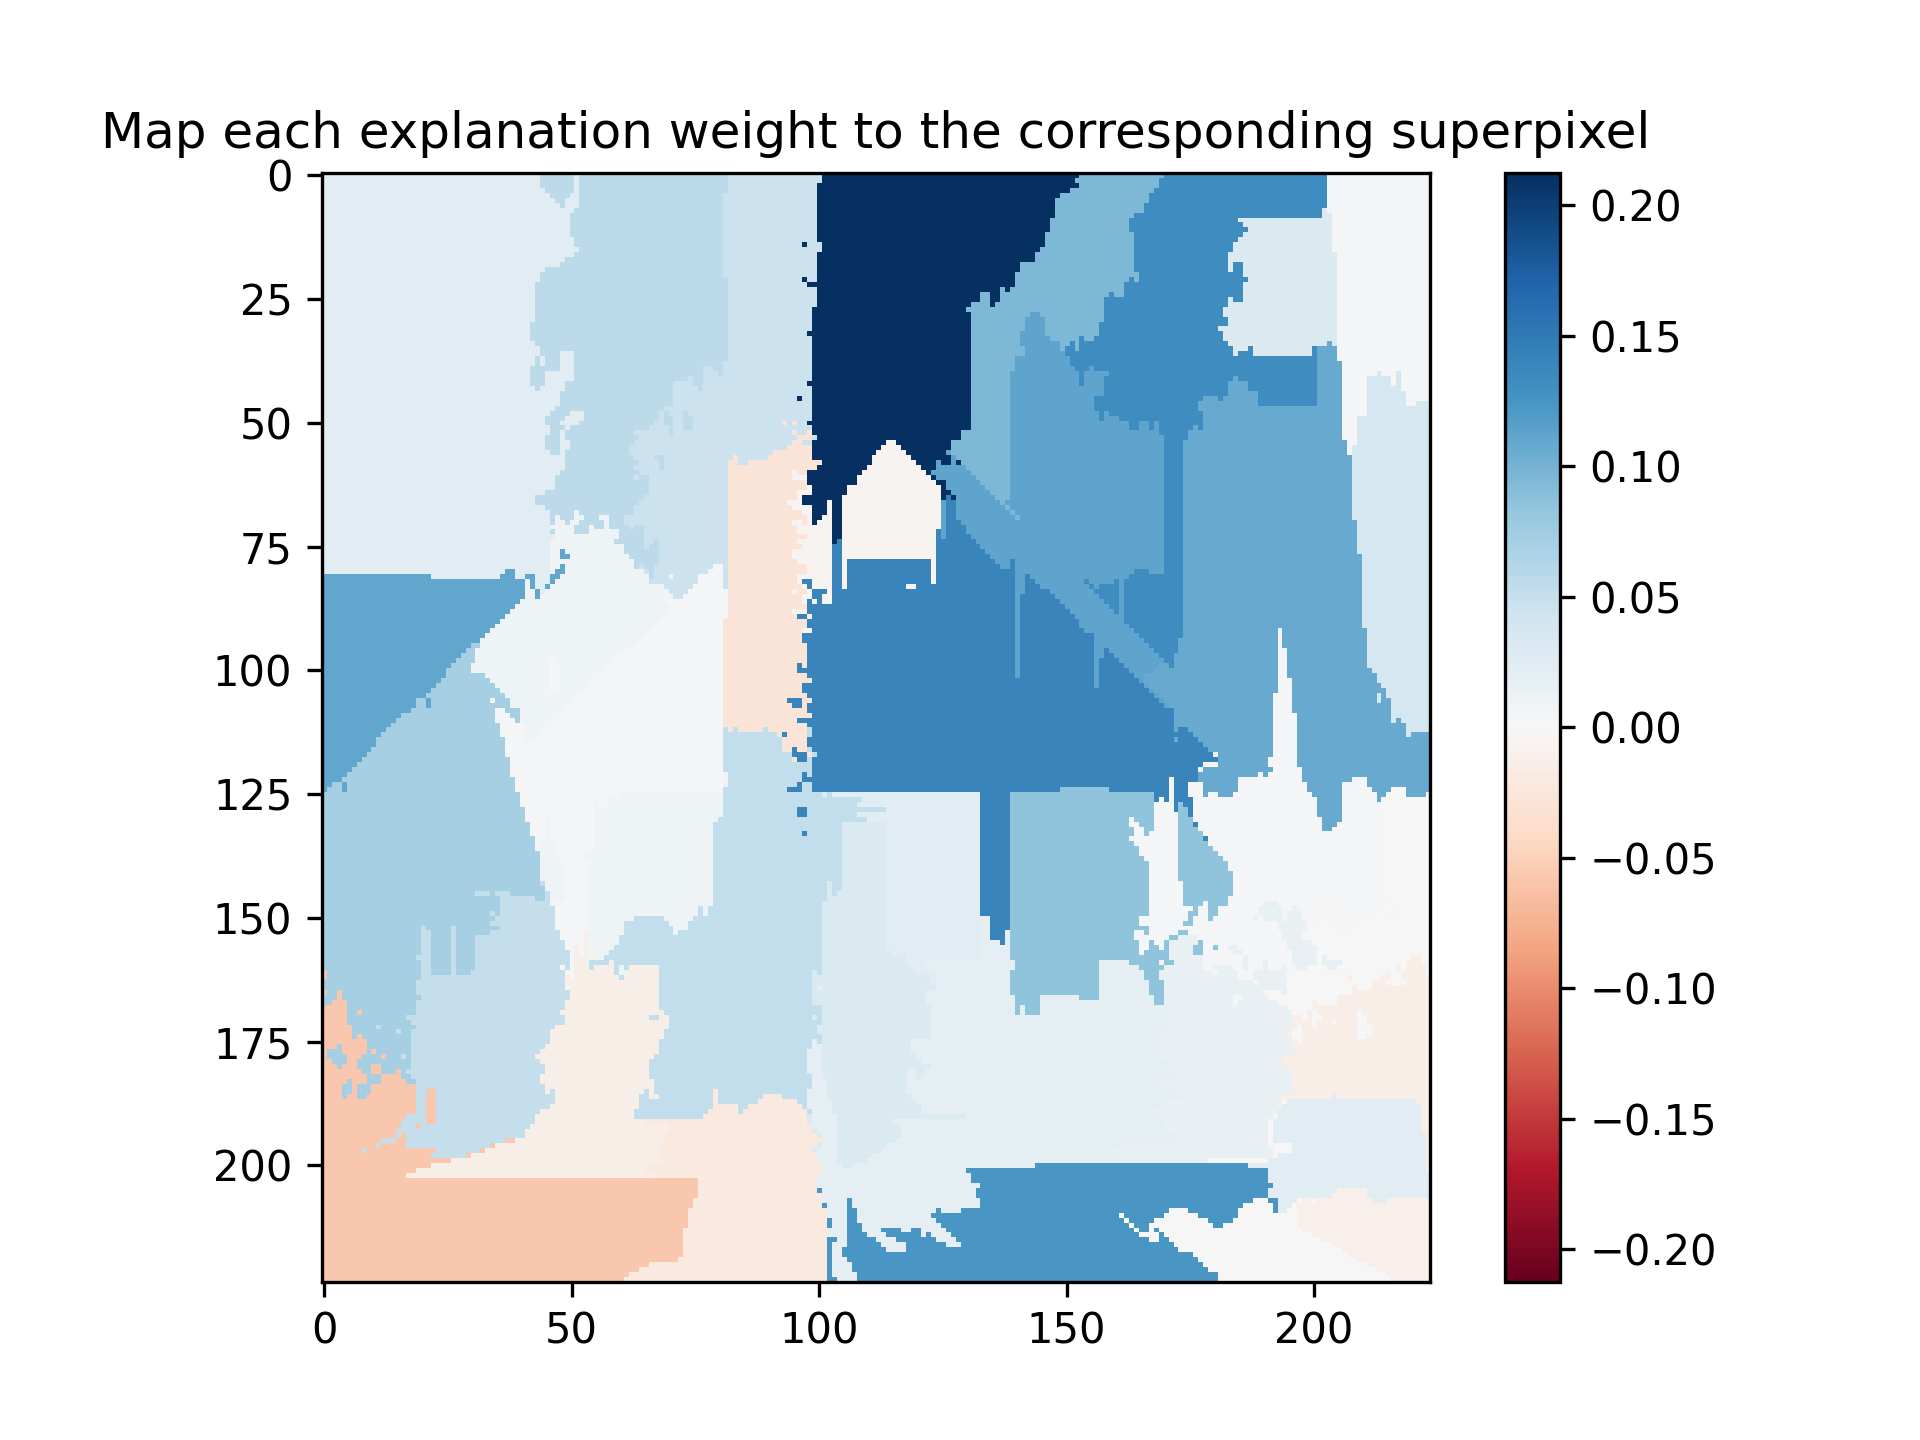
\includegraphics[width=0.49\linewidth]{lame_1_Map each explanation weight to the corresponding superpixel.png}
    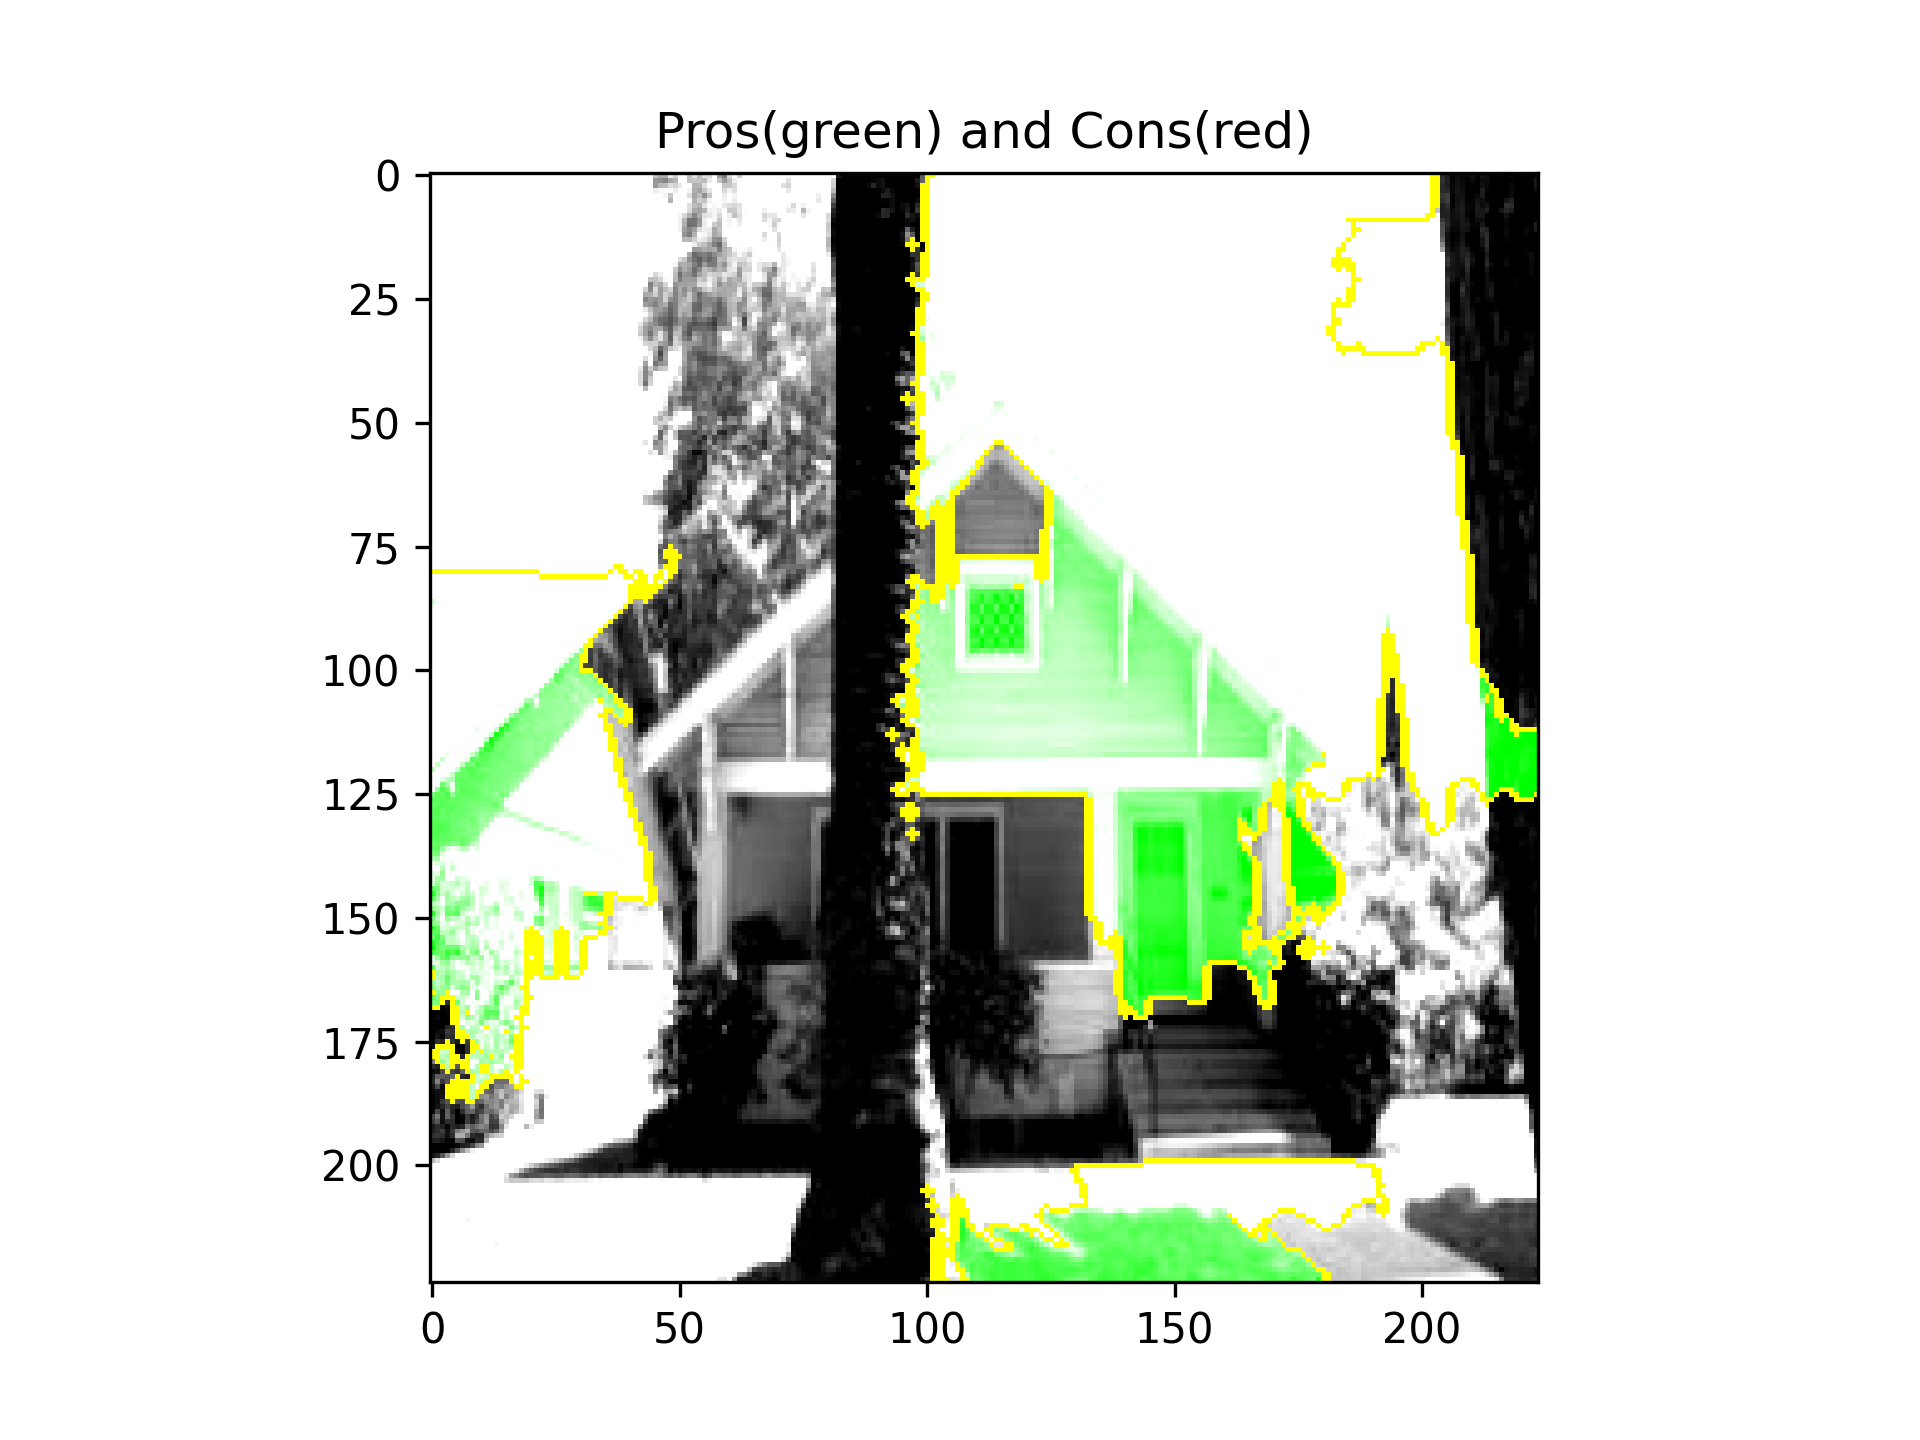
\includegraphics[width=0.49\linewidth]{lame_1_Pros(green) and Cons(red).png}
    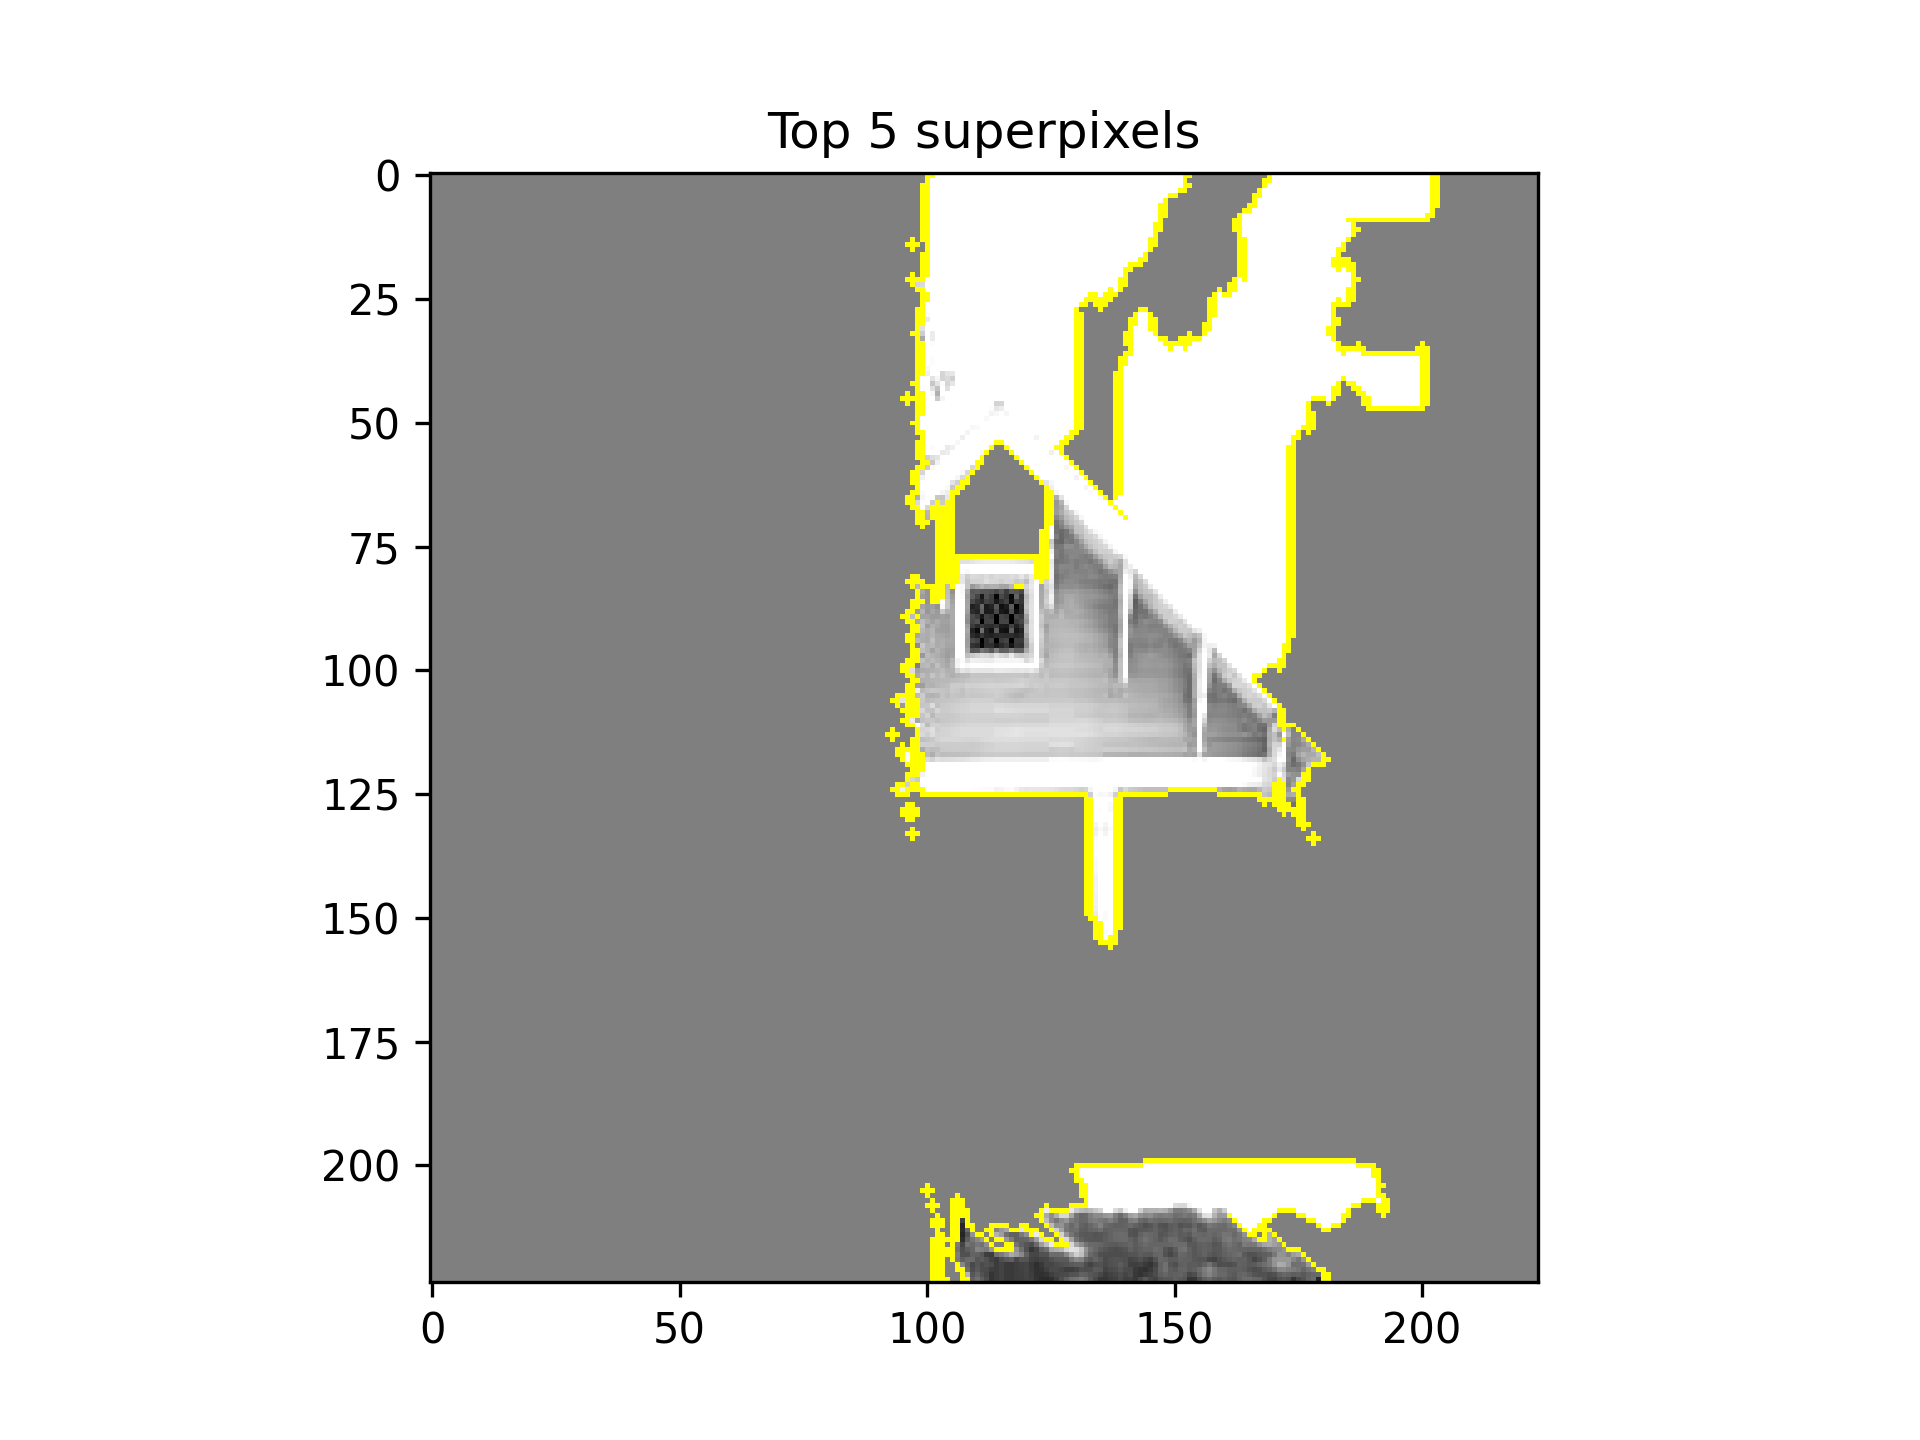
\includegraphics[width=0.49\linewidth]{lame_1_Top 5 superpixels.png}
    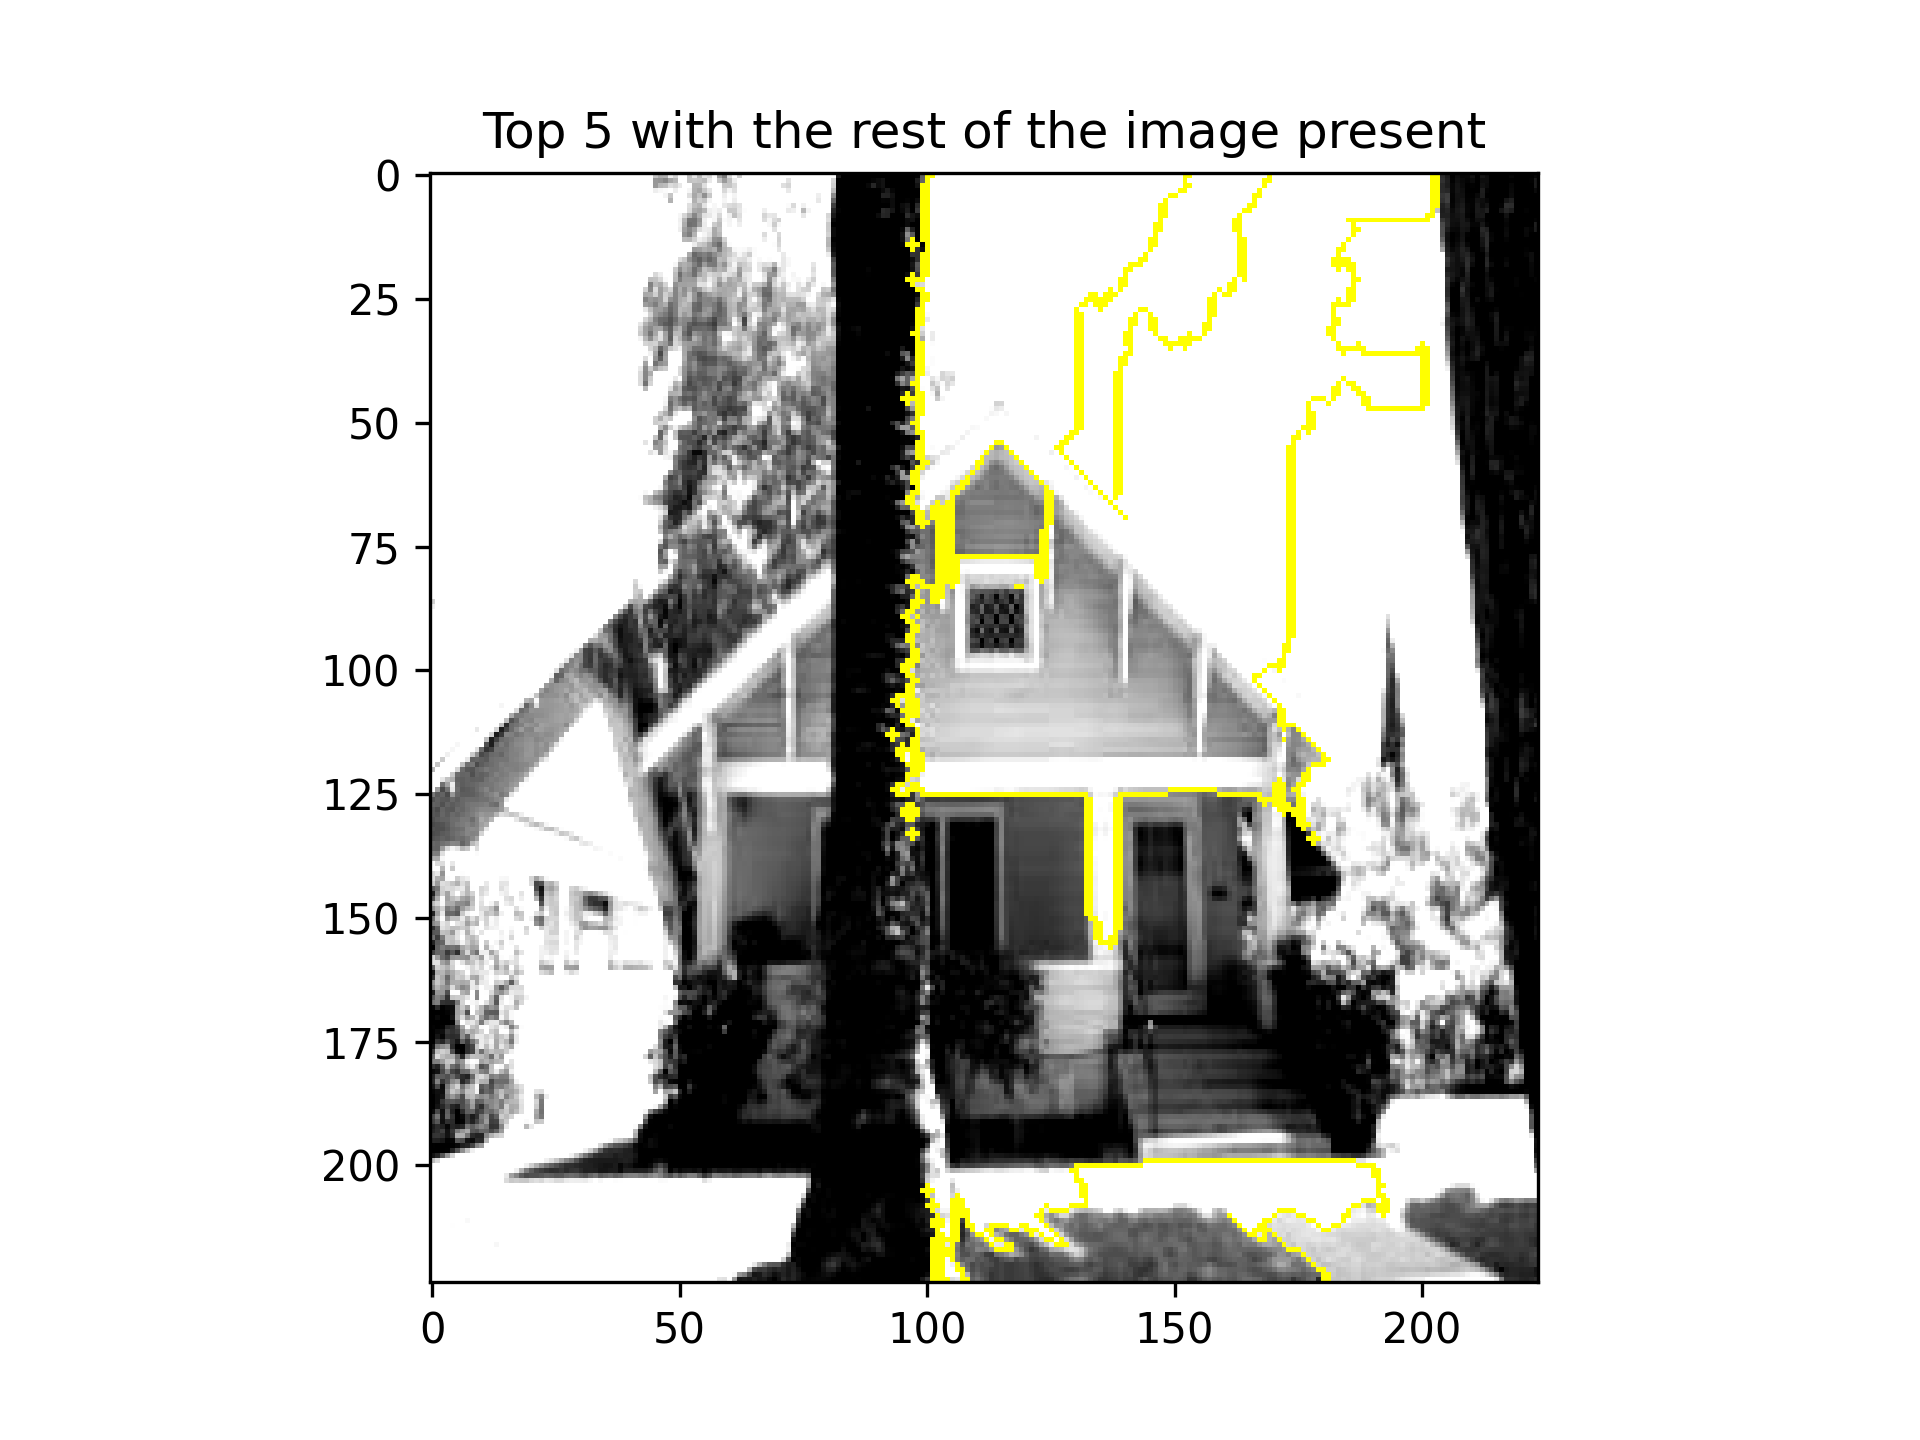
\includegraphics[width=0.49\linewidth]{lame_1_Top 5 with the rest of the image present.png}
    \caption{LIME plots for the first falsely categorized image, predicted as \emph{Tall building} but ground truth is \emph{Suburb}}
    \label{fig:LIME_1}
\end{figure}

\emph{Example 1}: The LIME plots are shown in Fig. \ref{fig:LIME_1}. The image is falsely classified as \emph{Tall building} while the ground truth label is \emph{Suburb}. From the LIME plots, we could see that superpixels are mainly focused on the building and ignored the environment. That is why the model would classify this image into \emph{Tall building} rather than \emph{Suburb}.


\emph{Example 2}: The LIME plots are shown in Fig. \ref{fig:LIME_2}. The image is falsely classified as \emph{Open Country} while the ground truth label is \emph{Highway}. From the LIME plots, we could see that superpixels are mainly focused on the sky and wide ground. It ignores a large part of the highway. That is why the model would classify this image into \emph{Open Country} rather than \emph{Highway}.

\begin{figure}[htbp]
    \centering
    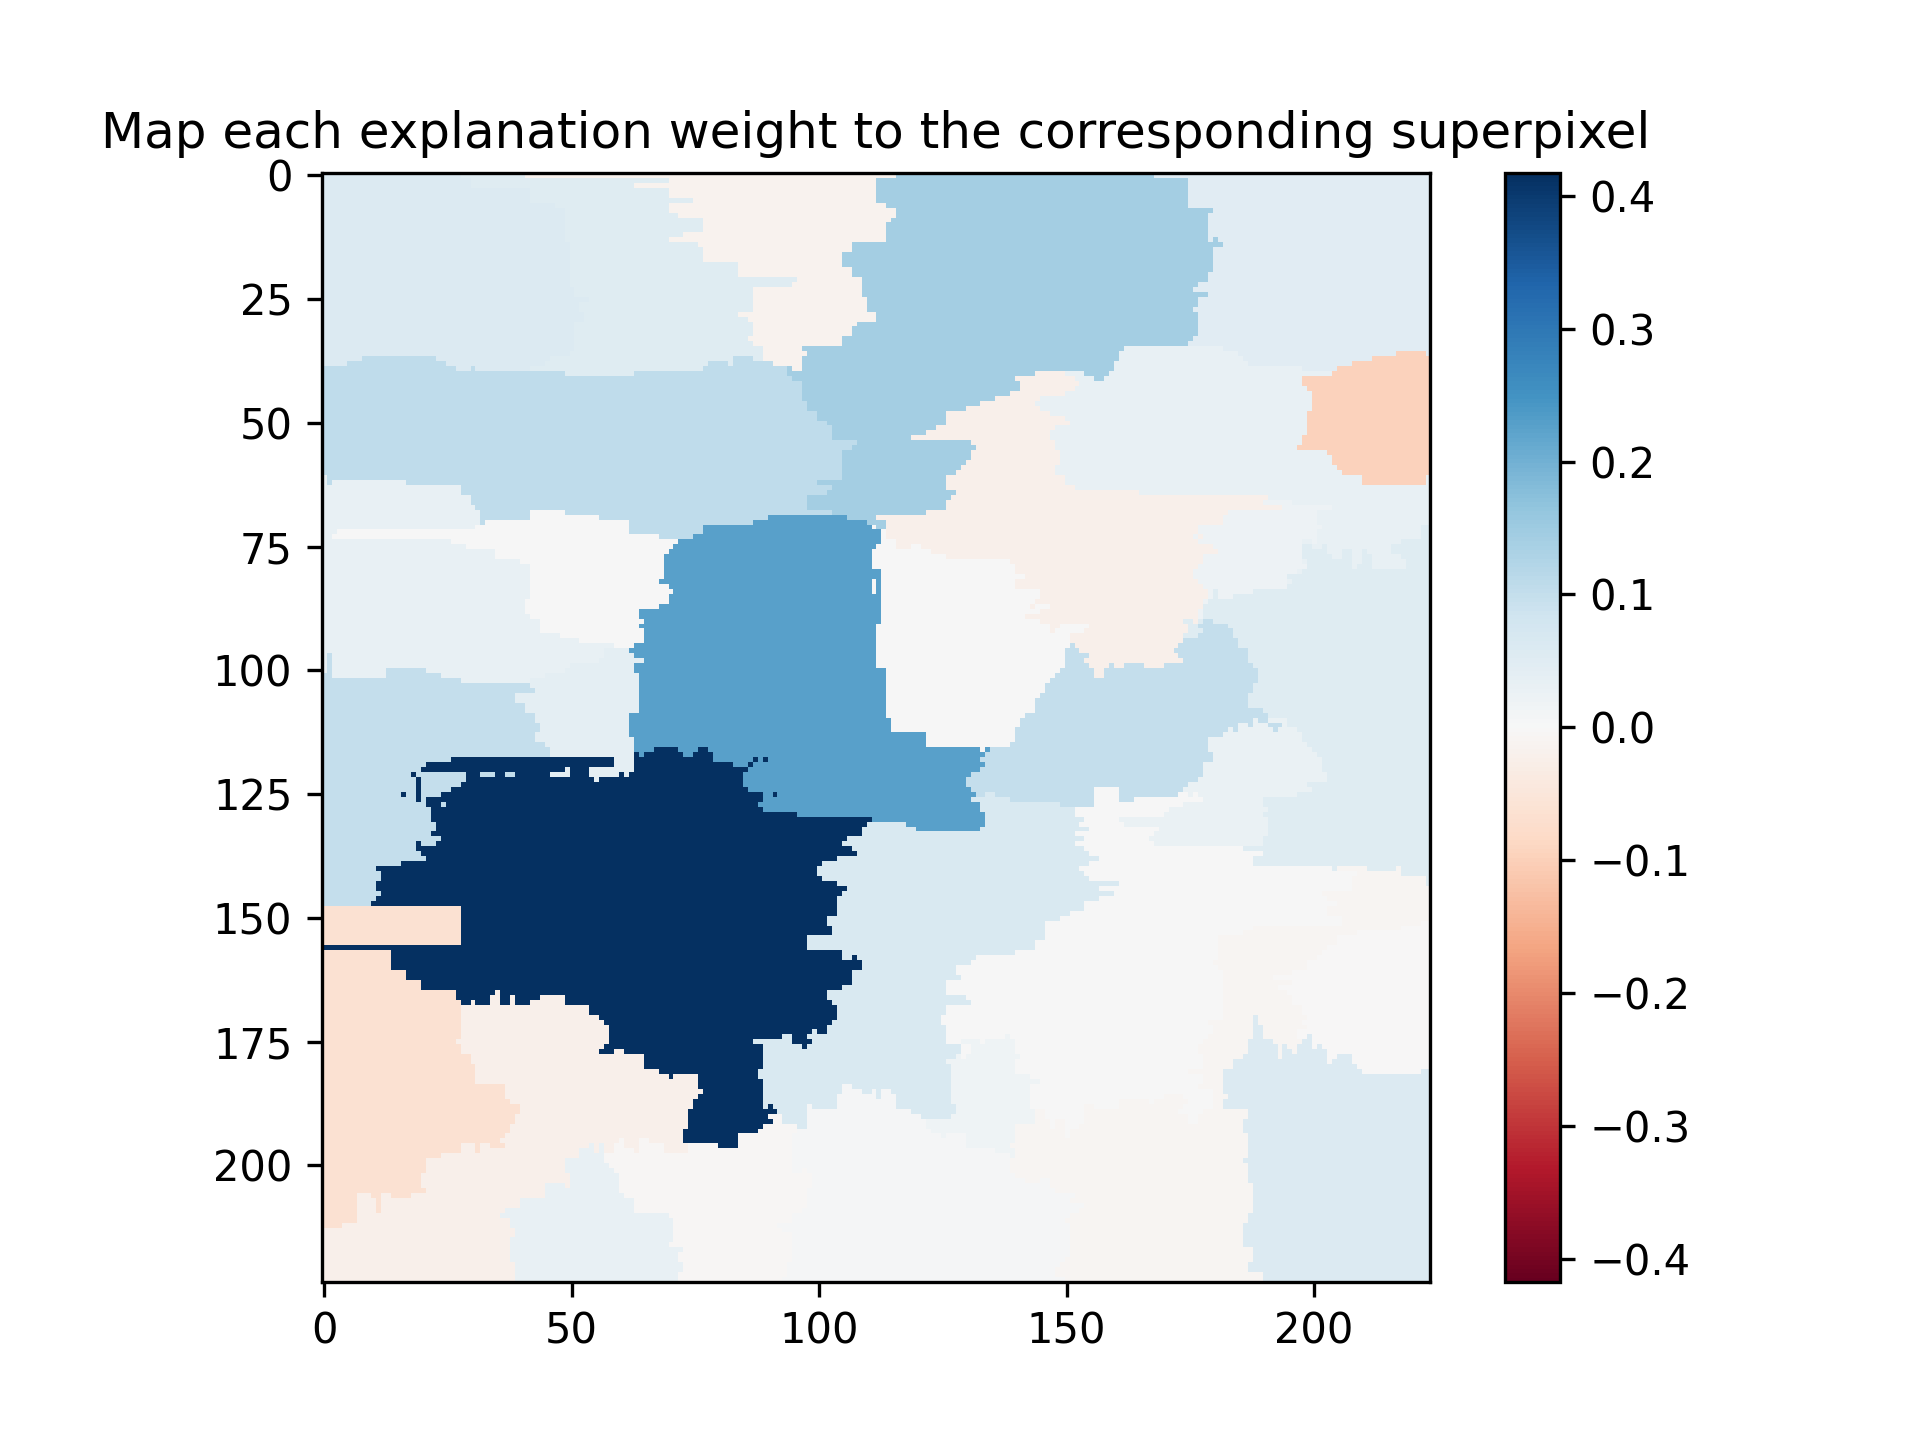
\includegraphics[width=0.49\linewidth]{lame_2_Map each explanation weight to the corresponding superpixel.png}
    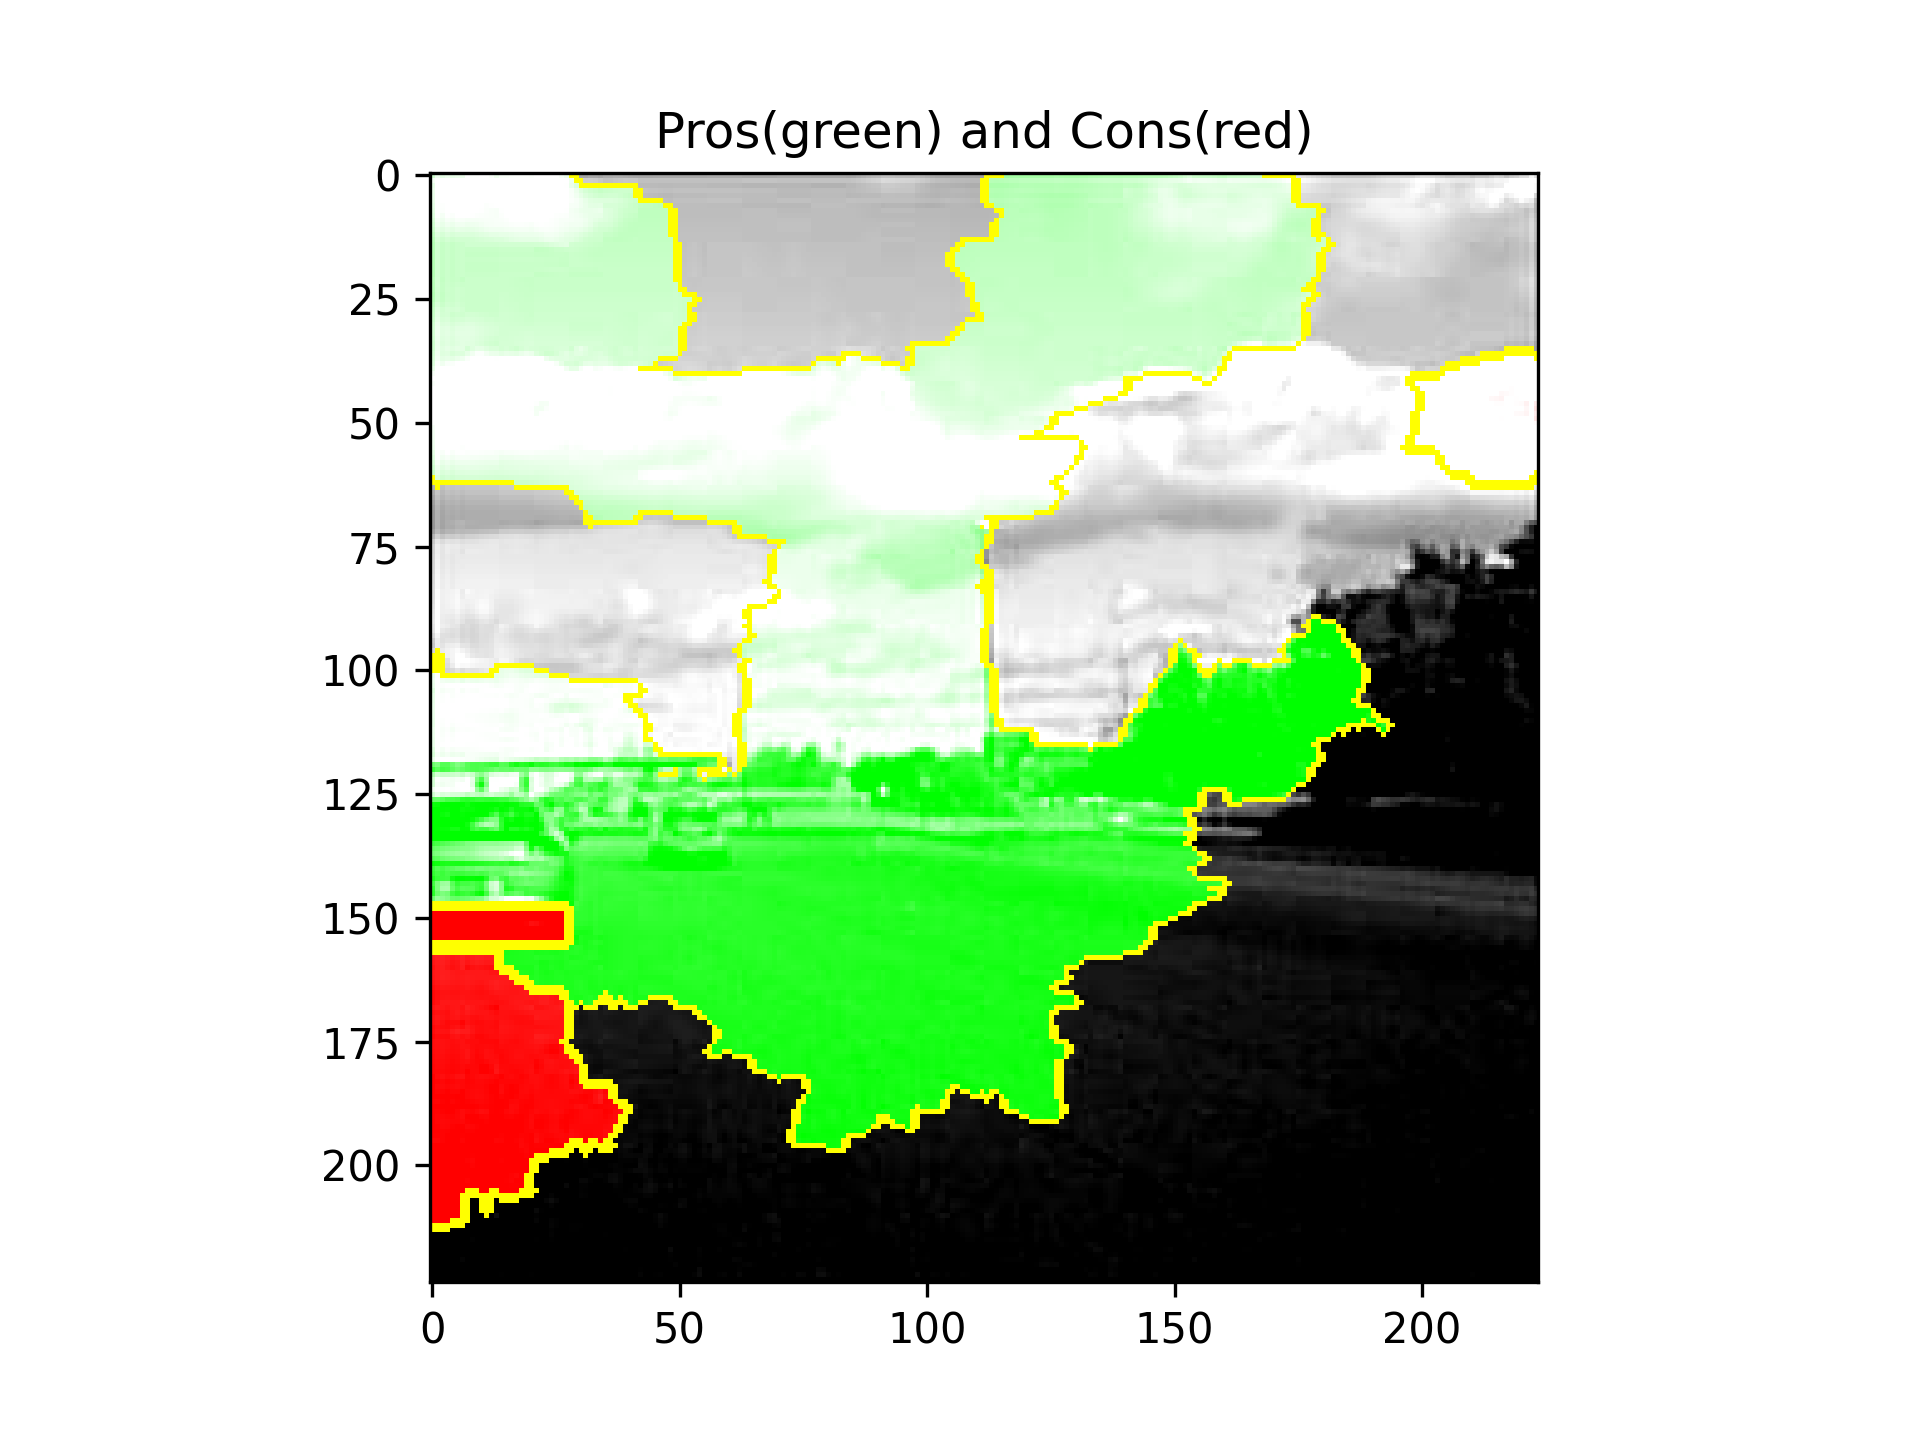
\includegraphics[width=0.49\linewidth]{lame_2_Pros(green) and Cons(red).png}
    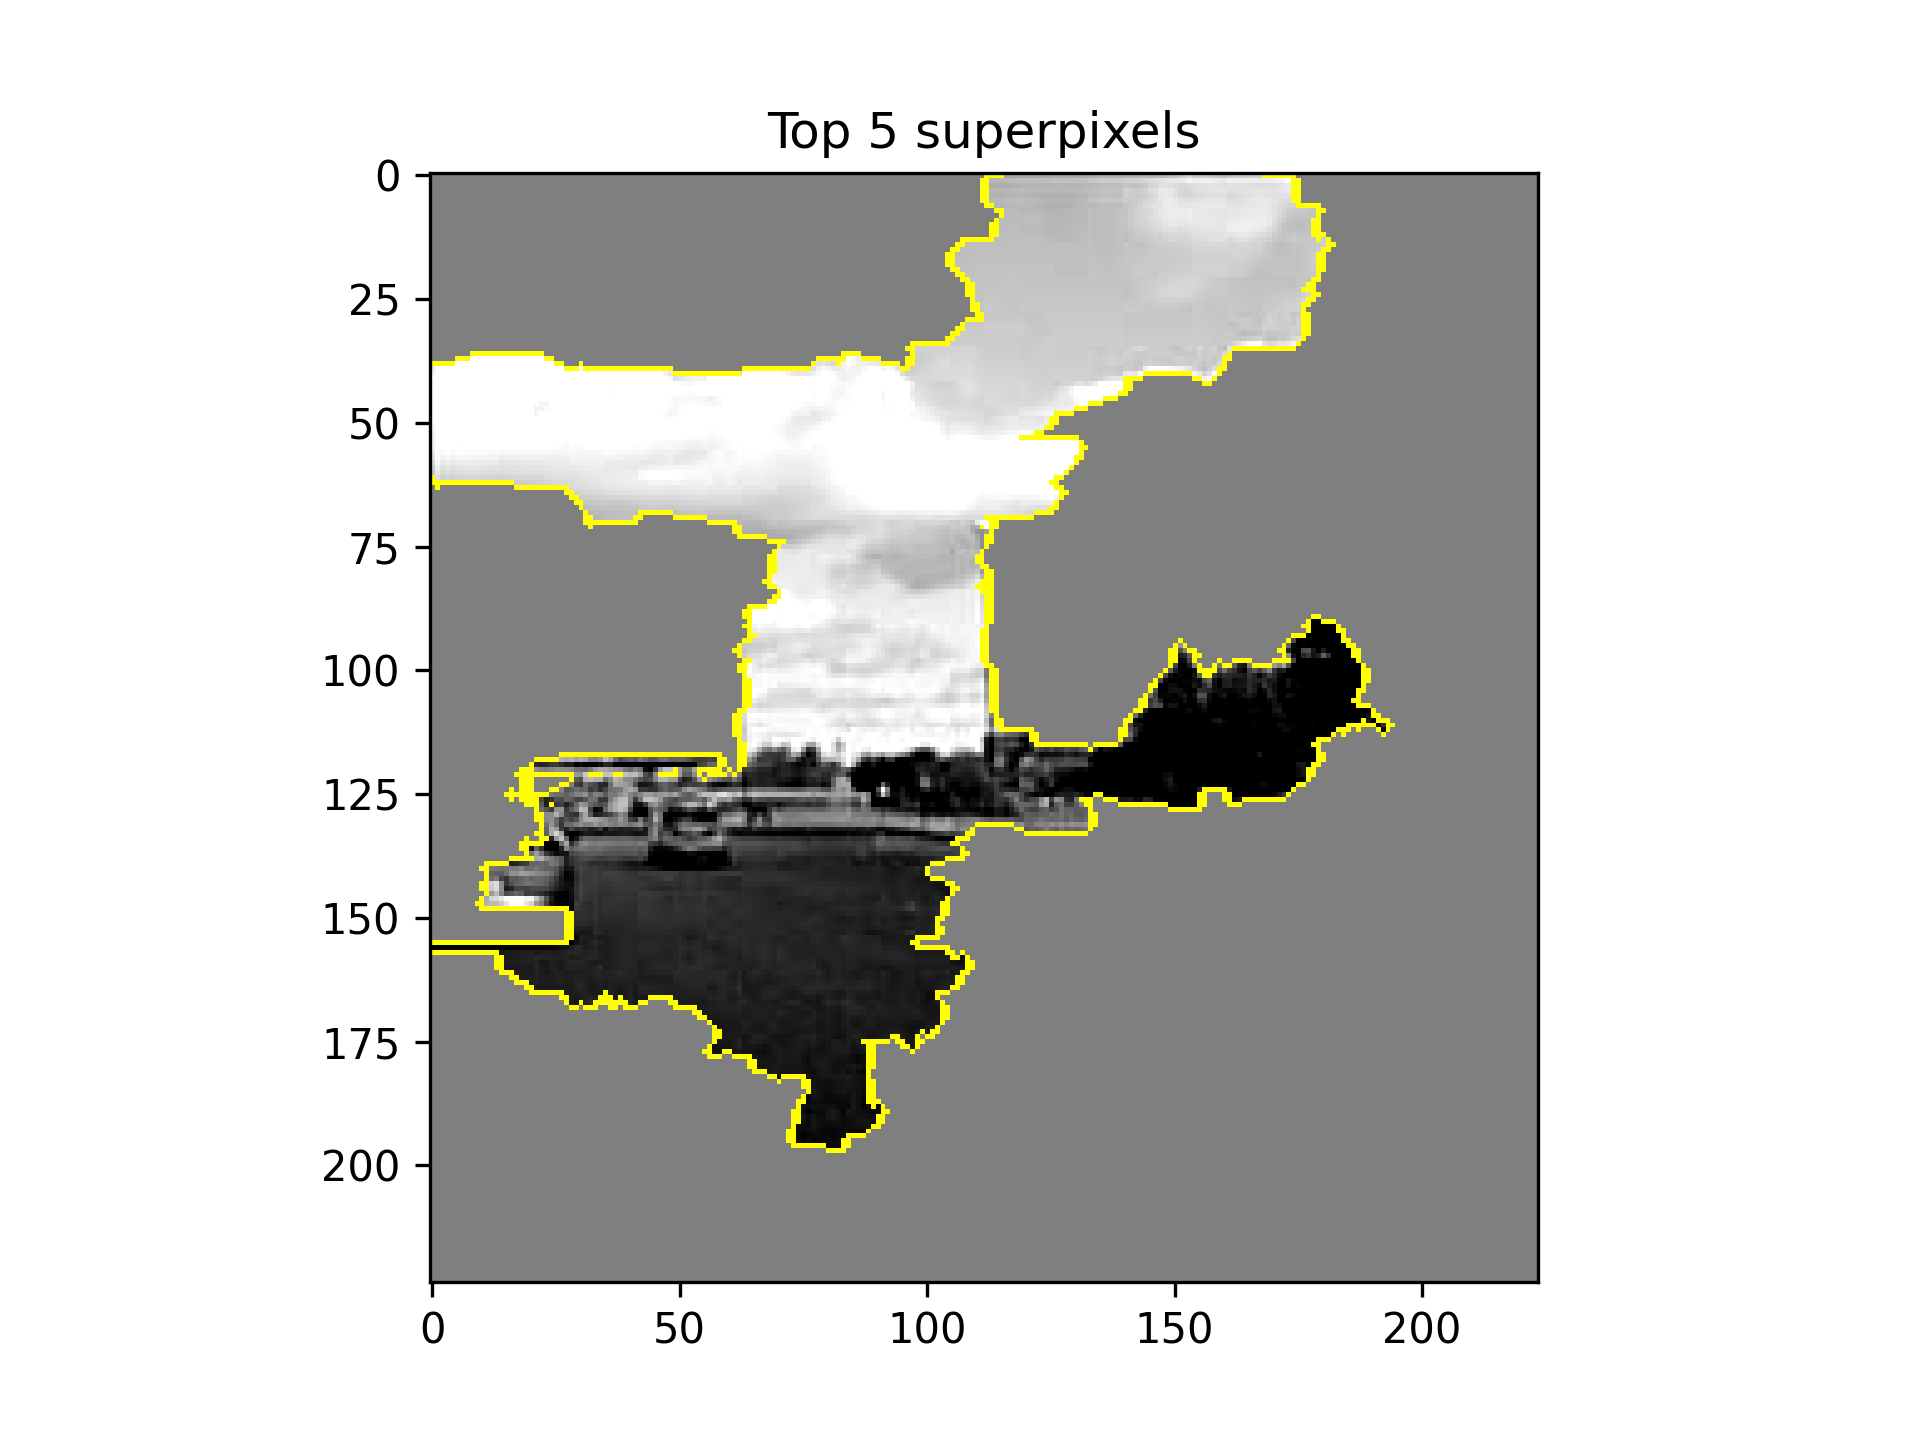
\includegraphics[width=0.49\linewidth]{lame_2_Top 5 superpixels.png}
    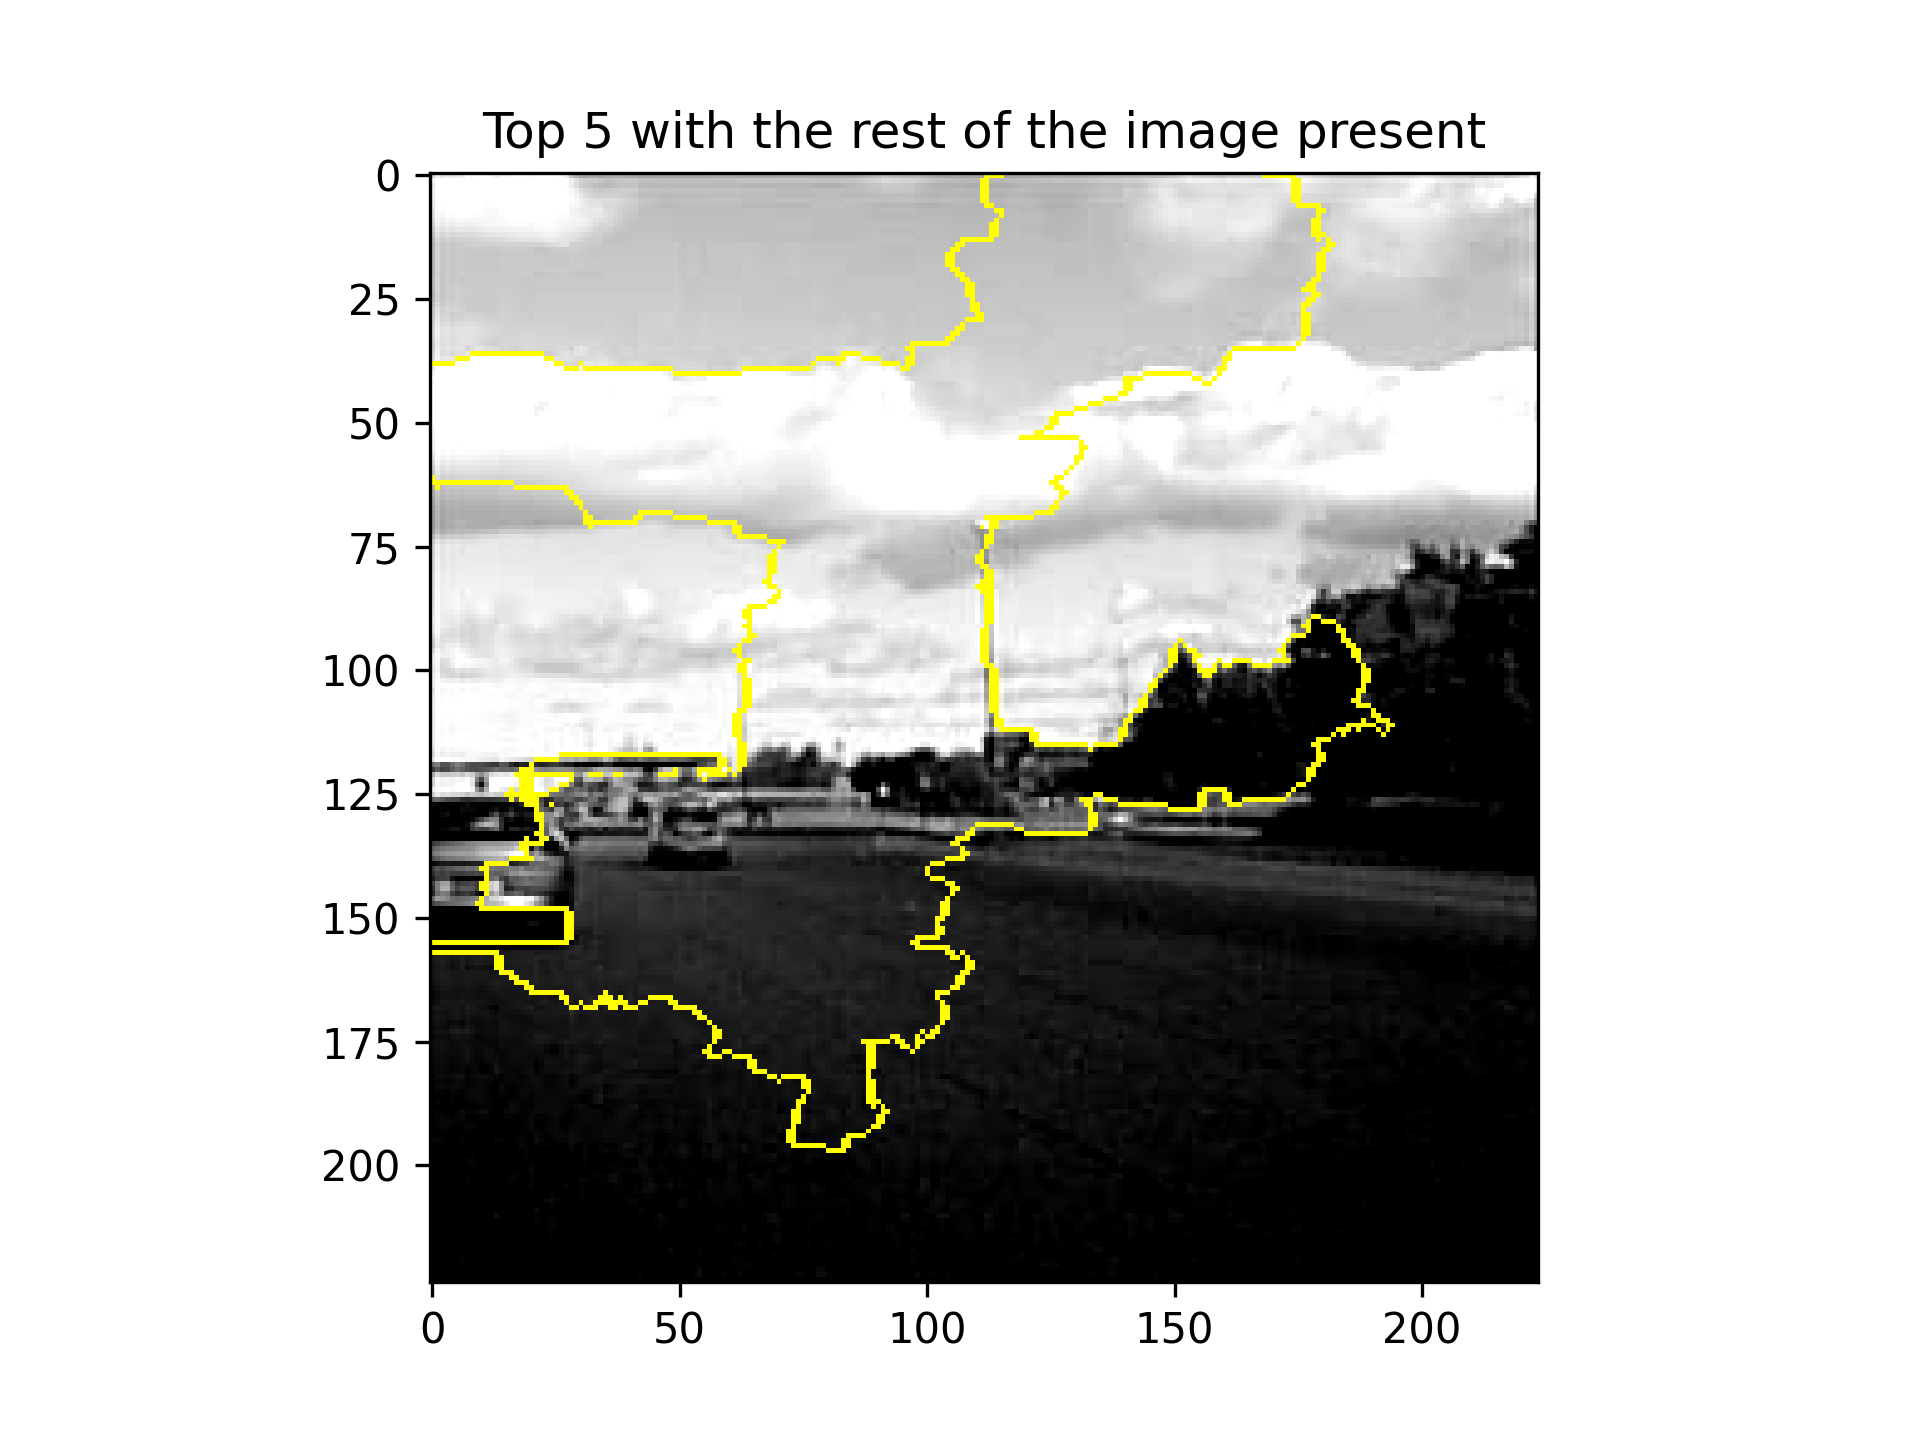
\includegraphics[width=0.49\linewidth]{lame_2_Top 5 with the rest of the image present.png}
    \caption{LIME plots for the second falsely categorized image, predicted as \emph{Open Country} but ground truth is \emph{Highway}}
    \label{fig:LIME_2}
\end{figure}

\subsection*{Task 3}

\emph{Vgg\_head}: To make the model be able to classify scences, we first need to flatten the CNN layers, which is followed by two fully-connected layers with BatchNormalization and Dropout layer respectively to avoid overfitting. The final layer is a fully-connected layer with neuron number as the number of classes. The activation functions for each layer are relu except for the final layer, which is softmax to calculate the prediction probability.
    \begin{python}
self.optimizer = tf.keras.optimizers.Adam(hp.learning_rate)

self.head = [
    Conv2D(256, 1, 1, padding='same', activation='relu'),
    GlobalAveragePooling2D(),
    Dropout(rate=0.5),
    Dense(hp.num_classes, activation="softmax"),
  ]
  
### loss definition
loss = tf.keras.losses.sparse_categorical_crossentropy(labels, predictions)
    \end{python}

\section*{Result}

The model summary are presented in Fig. \ref{fig:your_model_summary} and Fig. \ref{fig:vgg_summary}. The graphs of loss function over time during training are presented in Fig. \ref{fig:your_model_results} and Fig. \ref{fig:vgg_results}.

After implementing the model structures described above and hyperparameters optimization, the best achieved performance of \emph{your\_model} is 75\% and VGG is 91\%. The classification performance for each step of two models are plotted in Fig. \ref{fig:your_model_results} and Fig. \ref{fig:vgg_results}.

\begin{figure}[htbp]
    \centering
    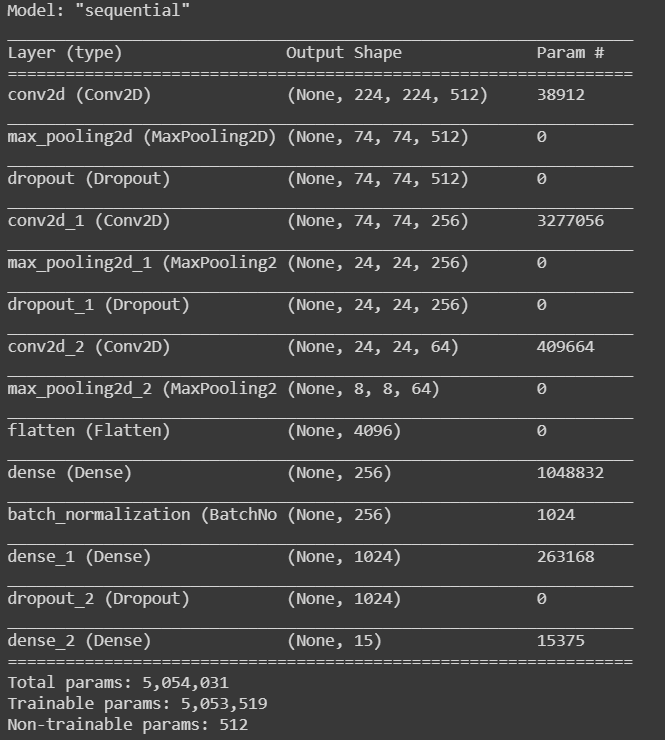
\includegraphics[scale=0.8]{your_model.png}
    \caption{screenshot of your\_model summary}
    \label{fig:your_model_summary}
\end{figure}

\begin{figure}[htbp]
    \centering
    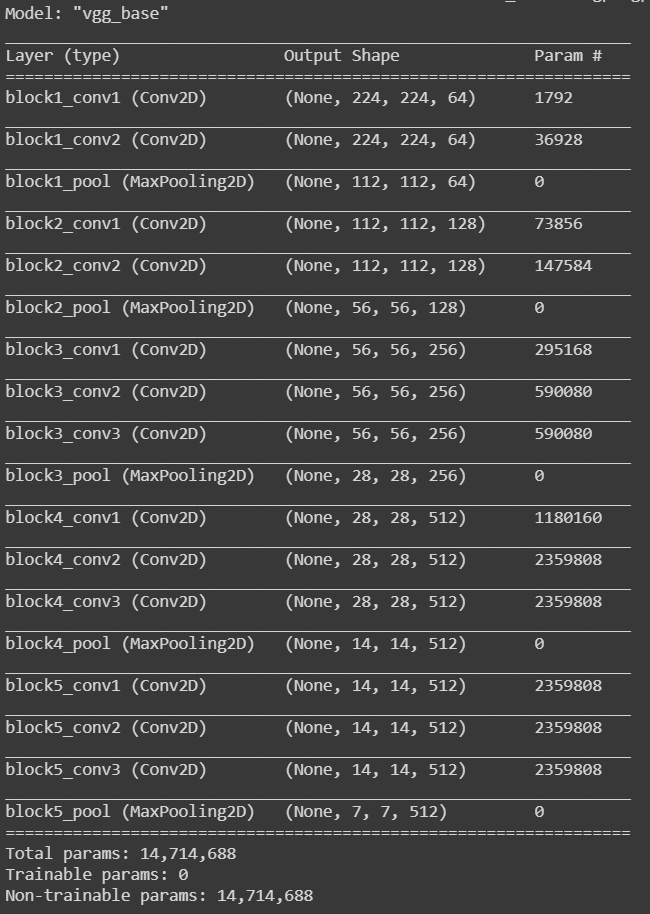
\includegraphics[scale=0.65]{vgg_1.png}
    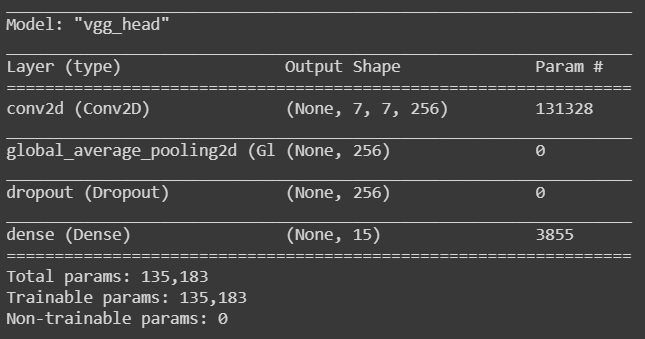
\includegraphics[scale=0.65]{vgg_2.png}
    \caption{screenshot of VGG model summary}
    \label{fig:vgg_summary}
\end{figure}

\begin{figure}
    \centering
    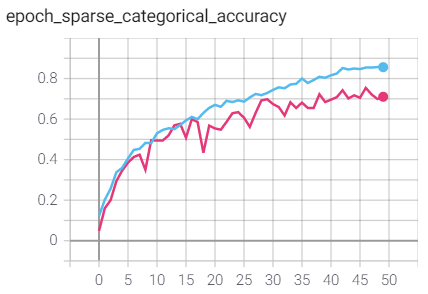
\includegraphics[]{your_model_batch_acc.png}
    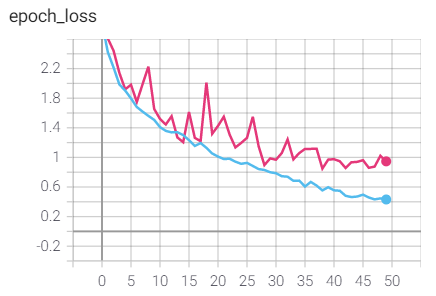
\includegraphics[]{your_model_epoch_loss.png}
    \caption{\emph{Above}:classification performance for each step in your\_model. \emph{Below}: your\_model loss function over time during training}\
    \label{fig:your_model_results}
\end{figure}


\begin{figure}
    \centering
    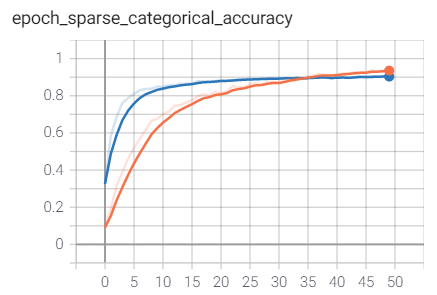
\includegraphics[]{vgg_batch_acc.png}
    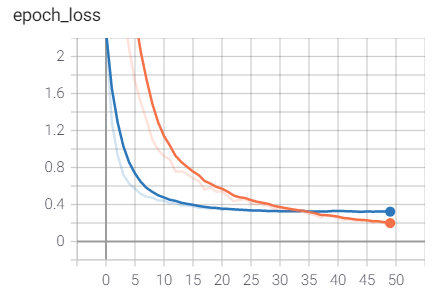
\includegraphics[]{vgg_epoch_loss.png}
    \caption{\emph{Above}:classification performance for each step in VGG. \emph{Below}: VGG loss function over time during training}
    \label{fig:vgg_results}
\end{figure}


% \section*{Extra Credit (Optional)}
% \begin{enumerate}
%     \item Gather additional scene training data (e.g., from the SUN database or the Places database) and train a network from scratch. Report performance on those datasets and then use the learned networks for the 15 scene database with fine tuning.

%     \item up to 10 pts: Try a completely different recognition task. For example, try to recognize human object sketches (download the .png files).
% \end{enumerate}

\end{document}
